\chapter{BayesQuant: Probabilistic estimation of protein ratios}
\label{chap:model}

\section*{Summary}

The current label-free quantification methods reviewed in section \ref{sec:quantification} rely on frequentist statistics, which return point estimates of model parameters such as the estimate of the abundance ratio (fold change) across conditions. However, a Bayesian  approach to this problem, that we know of, is lacking in the literature. As a response to this shortcoming, a statistical model, named BayesQuant, was written in the probabilistic programming framework PyMC3 and tested on the same benchmark dataset from chapter \ref{chap:pipeline}). The execution of the three steps required when doing Bayesian modelling, mainly (I) model implementation, (II) computation of posterior probabilities and (III) model checking, will be described for this particular problem in the present chapter, together with a discussion on its usability, its strengths and its weaknesses.

\section{Introduction}

\subsection{Frequentist and Bayesian statistics}

Both the LFQ and MSqRob quantitication engines presented in chapter \ref{chap:pipeline} took a frequentist approach to the problem of protein quantification. Such approaches, establish a null hypothesis $H_0$, complementary to the actual hypothesis being tested (alternative hypothesis $H_1$). The information about the phenomena being modelled is put to use to measure how likely this null hypothesis is via Null-Hypothesis Significance Testing (\ac{NHST}).


\begin{align}
H_0: & \log_2(FC) = 0 \nonumber \\
H_1: & \log_2(FC) \neq 0 \nonumber
\end{align}

The results of this analysis will depend not only of the observed data, but also the data generation process \cite{Kruschke}. This way, both tools returned point estimates of the log2FC between a pair of conditions and a p-value, which provides a measurement of the probability of the null hypothesis. The null hypothesis usually states that the true value of the parameter is 0. Thus, p-values do not say anything about the probability of the alternative (our) hypothesis.

The Bayesian statistical framework provides an alternative point of view by revolving the role played by the model parameters and the observed data. While frequentist statistics treats the data as random and the parameters as fixed, a Bayesian framework swaps their roles and yields a probability distribution for any model parameter given the provided data. Bayesian analyses rely on the observed data and prior knowledge about the phenomenon only, and comes equipped with an equation that mathematically formalizes how to introduce these two dependencies in a valid way. This is the so called Bayes\textquotesingle s theorem.

\begin{equation}
P(\theta | y) = \cfrac{P(y | \theta) P(\theta)}{P(y)}
\end{equation}

The Bayes theorem is an extremely versatile tool taking a role analogous to that of statistics like T, F, or $\chi^2$. Unlike them, which are tailored to specific scenarios, it can be used to compute the probability distribution of almost any parameter in any model. 4 terms can be distinguished in its expression

\begin{enumerate}

\item $P(\theta)$: the \textbf{prior} probability distribution of the model parameter, introduces previous knowledge about the phenomenon being modelled.

\item $P(y | \theta)$: the probability distribution of the observed data (y) over the possible parameter space. It is also known as \textbf{likelihood} of the model, and its duty is updating our beliefs about the phenomenon by capturing the information in the data.

\item $P(y)$: the probability of the data, defined as the marginal probability of the data given a parameter value, for all possible values. It acts as a normalizing constant that makes the resulting distribution a true probability distribution adding up to 1. It is also known as the data \textbf{evidence}.

\item $P(\theta | y)$: the updated probability distribution of the model parameter, with the information extracted from the observed data. Since it reflects the beliefs about the phenomena after observing data, it is called \textbf{posterior} probability distribution,as opposite to the prior.

\end{enumerate}


The Bayes\textquotesingle s theorem formulated above is thus read as \textit{the posterior probability of the parameter $\theta$ is equal to the \textbf{prior} probability distribution times the likelihood divided by a constant}.

It can be applied to the quantification problem, where $\theta$ turns into the log2FC parameter we try to estimate. All is needed is the computation of the posterior probability distribution. Unfortunately, this is tractable analytically for simple models only. However, Markov Chain-Monte Carlo (\ac{MCMC}) and Variational Inference (\ac{VI}) methods can be used to approximate this posterior. Both of which are now possible to run thanks to the advent of modern computing.

\subsection{Inference methods: \ac{MCMC} and \ac{VI}}

The posterior distribution can be approximated (inferred) by means of \ac{MCMC} and \ac{VI} methods. On the one hand, \ac{MCMC} methods simulate sampling from the posterior distribution by constructing an ergodic Markov chain on $\theta$ whose stationary distribution is the posterior p($\theta$ | y) \cite{Blei2017}. Monte Carlo sampling is performed on the Markov Chain, (hence the name of the technique) to randomly explore the parameter space with some heuristics. This heuristic guarantees convergence of the empirical estimate with the true posterior, provided a big enough sample size. Sampling convergence is defined as the status reached by the sampler when it estimates a distribution of probability that does not change anymore, regardless of how much longer the sampler runs \cite{Tran2018} \footnote{\href{http://www.cs.jhu.edu/~jason/tutorials/variational.html}{http://www.cs.jhu.edu/~jason/tutorials/variational.html}}. The first sampling algorithms, like Metropolis-Hastings \cite{Chib1995} \footnote{A very nice tutorial on how Metropolis-Hastings works \href{http://twiecki.github.io/blog/2015/11/10/mcmc-sampling/}{http://twiecki.github.io/blog/2015/11/10/mcmc-sampling/}} \footnote{Likewise, this resource provides very illustrative explanations of Hamiltonian-MC and NUTS \href{http://elevanth.org/blog/2017/11/28/build-a-better-markov-chain/}{http://elevanth.org/blog/2017/11/28/build-a-better-markov-chain/}} have given way to the much more efficient sampler \ac{NUTS} \cite{Hoffman2011}.

On the other hand, \ac{VI} methods, very recently developed and introduced in PyMC3, provide a fast alternative to \ac{MCMC} methods, yet they are not guaranteed to asymptotically approximate the true posterior. In \ac{VI}, optimization, instead of sampling, is employed as way to approximate the posterior \cite{Blei2017}. More concretely, a family of densities $Q$ over the parameters $\theta$ is defined. The goal of \ac{VI} is to find the single density $q$ within the family $Q$ that best approximates $p(\theta|y)$. This approximate density should be complex enough to reach a good approximation, and at the same time simple enough to be computationally easy to work with. The best candidate is defined as the one minimising the Kullback-Leibler (\ac{KL}) divergence (see equation \ref{eq:KL}).

\begin{gather}\label{eq:KL}
q^*(\theta) = \argmin \infdiv*{q(\theta)}{p(\theta|x)}
\end{gather}

where $q(\theta)$ stands for the whole family of densities, $p(\theta|x)$ stands for the true posterior and $KL$ stands for the \ac{KL} divergence. $q^*(\theta)$ is the best candidate density.

From \footnote{\href{http://www.cs.jhu.edu/~jason/tutorials/variational.html}{http://www.cs.jhu.edu/~jason/tutorials/variational.html}} \textit{the term variational is used because the best $q$ in $Q$ is picked. The term derives from the "calculus of variations," which deals with optimization problems that pick} [...] \textit{a particular $q$ in $Q$, specified by setting some variational parameters i.e the knobs on $Q$ that need to be turned to get a good approximation.}


One of the terms yielded by the decomposition of the conditional density embodied by the posterior is the evidence of the data $p(x)$.  $p(x)$ is computationally intractable, thus making the computation of the exact \ac{KL} divergence impossible. A lower bound up to an additive constant can however be computed thanks to Jensen\textquotesingle s inequality \cite{jensen1906fonctions} \. This approximate amount is the Variational or Evidence Lower BOund (\ac{ELBO}). \textit{The \ac{ELBO} is the negative \ac{KL} divergence of plus $logp(x)$, which is a constant with respect to $q(z)$. Thus maximizing
the \ac{ELBO} is equivalent to minimizing the \ac{KL} divergence} \cite{Blei2017}.

Finally, several density approximation families are available. The mean-field family of densities is one of the most simple, as it ignores all dependencies between latent variables, and treats them as independent. From \href{http://www.cs.jhu.edu/~jason/tutorials/variational.html}{http://www.cs.jhu.edu/~jason/tutorials/variational.html} the mean-field approximations works by \textit{pretending that the variables are just behaving that way "on their own." The mean-field method throws away all of the interactions}. A generic mean-field family member is shown in equation \ref{eq:mean_field}.

\begin{equation}\label{eq:mean_field}
q(\theta_1, ..., \theta_m) = \prod_{j=1}^{m}{q(\theta_j)}
\end{equation} 

The demanding computational cost of the \ac{MCMC} and \ac{VI} schemes has only been recently met by the power of modern computers, thus making the approach feasible.


\subsection{Model checking}
\label{subsec:model_checking}

However the posterior distribution is obtained, a proper Bayesian analysis is not finished without a model checking step that looks at potential problems happenning in the fitting step, and confirms the goodness of fit of the model to the data.

\begin{itemize}

\item Evidence for non-convergence must be collected. Albeit lack of evidence of non-convergence does not guarantee convergence, the existence of evidence definitely proofs it \cite{Kruschke}.

\item Neither reaching convergence nor the best \ac{VI} approximation guarantee that the fitted model actually captures the data generation process. Therefore, the true posterior could be a bad reflection of the natural process being model and the best approximation will not solve it. Posterior Predictive Checks are carried out to measure how well the model captured the data properties \cite{Kruschke}.

\end{itemize}




\subsection{Probabilistic programming}

The infrastructure providing the inference and model checking algorithms is available under several implementations in different programming languages, like R (JAGS \cite{Plummer}) and Python (PyMC3 \cite{Salvatier2016}). All these frameworks make use of a programming paradigm called \textbf{probabilistic programming}.


The management of uncertainty in statistics is done by means of probability distributions, which account for the possible values that a parameter could take, together with how likely they are. Probabilistic programming offers the framework to build complex statistical models by storing probability distributions as variables of the program. Moreover, probabilistic programming packages supply the tools needed to perform inference with these models by taking experimental evidence (data) and fitting the distributions to the data using Bayes\textquotesingle theorem. The fit of the model to the data entails the computation of the posterior probability distribution, which is tallied using algorithms provided with the probabilistic programming tool.

PyMC3 is a mature Python module dedicated to support probabilistic programming. It features   intuitive model specification syntax, modern and powerful \ac{MCMC} sampling algorithms like the No-U-Turn-Sampler (\ac{NUTS}) as well as Automatic Differentiation Variational Inference (ADVI) \footnote{\href{https://github.com/pymc-devs/pymc3}{https://github.com/pymc-devs/pymc3}}. Therefore, it provides the tools required to build a Bayesian model for the probabilisitc estimation of protein \ac{log2FC} in proteomics datasets, that is, together with an estimate of its uncertainty.


\subsection{Goals}

\begin{enumerate}

\item Develop a Bayesian model to estimate log2FC in proteomics datasets together with the uncertainty of the estimate.

\item Make it scalable and fast for usability in ordinary modern computers.

\end{enumerate}

\section{Materials and Methods}

\subsection{Data input}
\label{subsec:data_input}

The peptides.txt and proteinGroups.txt files produced by MaxQuant \cite{Cox2008} after the analysis of the dataset published in \cite{Cox2014} were used as input for the modelling algorithm when running without sequence modelling, and processed using the \texttt{preprocess\_MaxQuant()} and \texttt{MSnSet2protdata()} functions in the MSqRob \cite{Goeminne2016} package, similar to what was done in section \ref{subsec:database_preparation}.

Peptides missing in any of the samples available were dropped from the analysis.

The final state of the data is shown in table \ref{tab:data_model} for a single protein.

\begin{table}
\begin{tabular}{llrrrrrr}
\toprule
protein &      Organism &     H1 &     H2 &     H3 &     L1 &     L2 &     L3 \\
\midrule
 P0A8I8 &       E. coli &  25.13 &  25.24 &  24.39 &  21.71 &  22.67 &  22.40 \\
 P0A8I8 &       E. coli &  21.49 &  23.10 &  23.38 &  21.34 &  22.65 &  21.25 \\
 P0A8I8 &       E. coli &  24.10 &  24.54 &  23.81 &  19.88 &  20.87 &  20.30 \\
 A6NDG6 &  Homo sapiens &  25.08 &  24.98 &  23.83 &  22.54 &  22.52 &  24.96 \\
 A6NDG6 &  Homo sapiens &  22.70 &  24.32 &  23.00 &  22.29 &  23.27 &  23.91 \\
 A6NDG6 &  Homo sapiens &  21.18 &  22.51 &  23.25 &  22.30 &  21.75 &  23.61 \\
\bottomrule
\end{tabular}
\caption[BayesQuant data input]{Sample data input for the Bayesian model. Every row represents a unique peptide. The first column refers to the protein it was found to map to in the protein inference step. The second column is an annotation field, in this case indicating the protein\textquotesingle s organism. The remaining columns indicate the $log_2(Intensity)$ registered for each peptide in the corresponding run. In this case, three peptides were observed for the proteins with ids \textit{P0A8I8} and \textit{A6NDG6}.}
\label{tab:data_model}
\end{table}

\subsection{Sequence feature extraction}

When running with active sequence modelling, the peptide sequences and their neighborhood in the protein was extracted from \textit{E. coli} and \textit{Homo sapiens} proteome databases (\ref{subsec:database_preparation}). The protein neighborhood was defined by a window spanning 15 aminoacids on both sides of the peptide. It was extracted using the seqinr \cite{Charif2007} and GenomicRanges \cite{Lawrence2013} packages implemented in R and Bioconductor.

Features to model the peptide effect based on sequence were extracted using the Biopython \cite{Cock2009} built-in  module \texttt{ProtParam.ProteinAnalysis()}. The following properties were extracted: amino-acid percentage, peptide length, molecular weight, mass/length ratio, isoelectric point, aromaticity and instability.

\subsection{Hierarchical modelling}
\label{subsec:hierarchy}


The \ac{MS1} intensity measurements are affected by two main sources of variation:

\begin{enumerate}
\item The fixed effect that the researcher aims at unraveling with proteomics (treatment effect)
\item Random noise produced by experimental procedures, sequence bias, etc, which lead to a loss of data quality and resolving power.
\end{enumerate}


A mass spectrometry-proteomics workflow aims at providing estimates of the treatment effect, upon which the biological interpretation of the results is done, while minimising the remaining unwanted effects. The mathematical framework implemented to model these effects was similar to the one used by MSqRob:

\begin{equation}\label{eq:model}
y_{ijkl} = \beta_{ijkl}^{0} + \beta_{ij}^{treatment} + \beta_{ik}^{peptide} + \beta_{il}^{run} + \epsilon_{i}
\end{equation}

where $y_{ijkl}$ stands for the $\log_2$-transformed intensity registered in treatment $j$, peptide $k$ and run $l$. This way, separate treatment, peptide and run effects are distinguished. $i$ stands for the protein index, which is evidently the same for all measurements belonging to peptides mapped to the same protein. $\epsilon$ models the noise that cannot be explained with the three effects aforementioned, and is the same for all measurements associated to the same protein.

For example, the measurement $y_{P,A,p,1}$ corresponds to a measurement mapped to protein $P$. The measurement is impacted by a fixed effect, produced by treatment $A$, but also the peptide effect in peptide $p$ and the run effect in run $1$. An intercept term was also added to account for the starting intensity value.

The data is thus affected by different effects acting independently, and in order to model them properly, multilevels need to be defined. Multilevel effects can be modelled with three approaches: pooled, unpooled, and hierarchically (see figure \ref{fig:multilevel}). Hierarchical modeling is used when the sampling variance is not the only source of variation among the parameters, but they still share a dependency. The intercept and the three effects were modeled as independent hierarchies.

\begin{figure}[H]
\centering
\begin{subfigure}{.9\textwidth}
\centering
\caption*{Pooled}
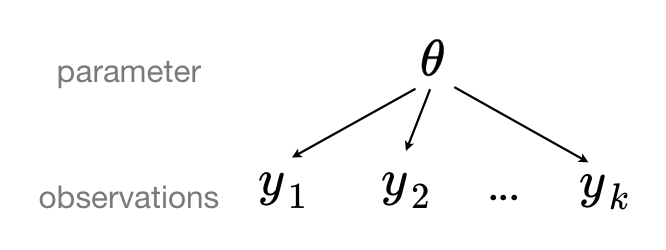
\includegraphics[width=0.85\linewidth]{model_pooled}
\end{subfigure}
\bigskip
\begin{subfigure}{.9\textwidth}
\centering
\caption*{Unpooled}
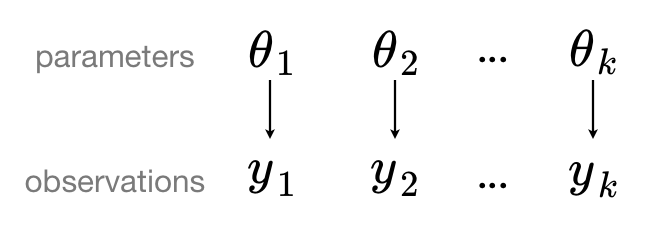
\includegraphics[width=0.85\linewidth]{model_unpooled}
\end{subfigure}
\bigskip
\begin{subfigure}{.9\textwidth}
\centering
\caption*{Hierarchical}
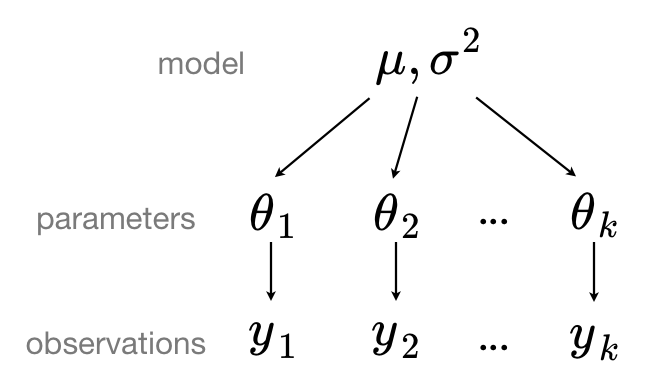
\includegraphics[width=0.85\linewidth]{model_hierarchical}
\end{subfigure}
\caption[]{Alternative multilevel modelling approaches. A pooled model assumes that the parameter distribution is the same for all the datapoints.  The unpooled model represents the opposite case, there every datapoint is assumed to be modelled by a different probability distribution of the parameter for each. Finally, a hierarchical model settles for a middle ground where the parameters will not be exactly the same but not completely different either. This is achieved by generating a global distribution from which the parameter for each datapoint is sampled \footnotemark{}.}
\label{fig:multilevel}
\end{figure}

\footnotetext{\href{https://docs.pymc.io/notebooks/multilevel\_modeling.html}{https://docs.pymc.io/notebooks/multilevel\_modeling.html}}


This way, independent and identically distributed (\ac{IID}) priors were set for the intercept, treatment, peptide and run effects. The particular effect observed on each peptide was then modelled as a value sampled from the corresponding \ac{IID} prior. A diagram of the resulting model is displayed in figure \ref{fig:daft_model}).

\begin{figure}[!h]
\centering
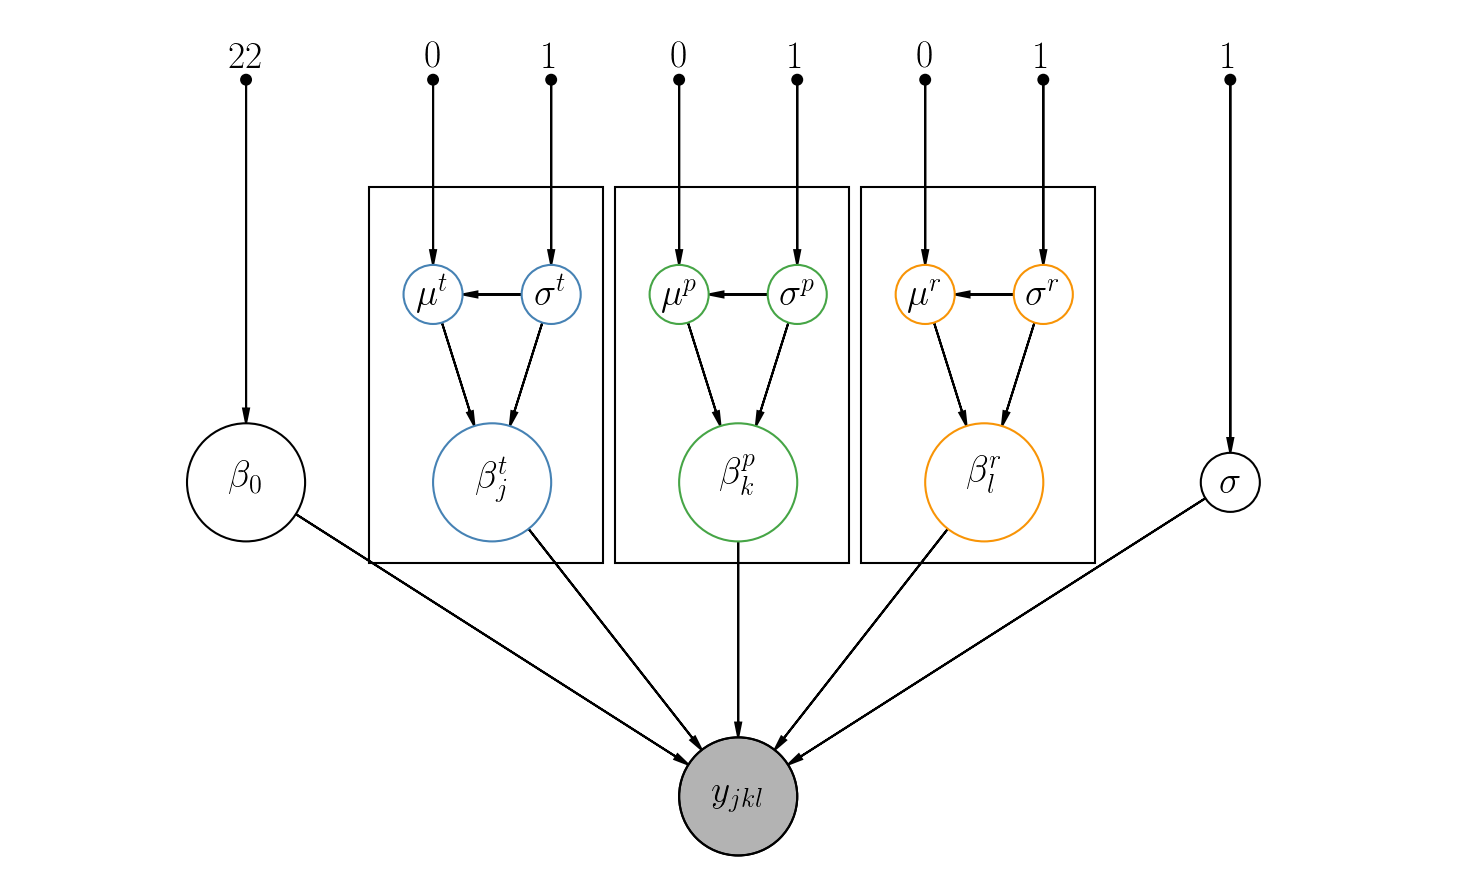
\includegraphics[width=\textwidth]{graph}
\caption[Bayesian model simplified diagram]{Diagram of the Bayesian model developed in the present work, without sequence modelling of the peptide effect. It is represented as a Directed Acyclic Graph (\ac{DAG}) where nodes represent hyperparameters or random variables (in a circle) and directed edges  represent the dependencies between them. The nodes on the top depict the hyperparameters of the model, governing the prior probability distributions represented by the nodes to which their edges lead to. The remaining nodes articulate the probabilistic model and all lead to a final node ($y_{ijkl}$) which represents the modelling of the observed data with the instantiated model. The model hierarchies are organized in boxes. The one corresponding to the treatment effect can be read as \textit{the treatment effect $\beta_{ij}^{t}$ observed in the data is modelled as a probability distribution conditional on the value of $\mu^t$ and $\sigma^t$, which are in turn probability distributions governed by the hyperparameters 0 and 1.}}
\label{fig:daft_model}
\end{figure}

\subsection{Prior probability distribution specification}

Both because of the little knowledge on the value of the parameters governing the data generation process and to provide a prior that everyone can agree upon, non informative priors were provided to the model. This was condensed in the specification of Normal and Half Normal distributions for all the random stochastic variables in the model. The hyperparameters were selected to be as non informative as possible.

\subsection{Posterior probability distribution computation}
\label{subsec:posterior_compute}

The \ac{VI} mean-field strategy was applied to approximate the posterior probability distribution of the \ac{log2FC}. \ac{ELBO} optimisation was run for 40k iterations. Optimisation was validated by visual inspection of \ac{ELBO} traceplots over the 40k iterations. Once optimisation was validated, 10k samples were drawn from the approximate distribution to simulate the true posterior.

\subsection{Model checking}

Posterior predictive checks of the posterior distribution were carried out using the \texttt{sample\_ppc()} function in PyMC3. 500 datapoints for each peptide, consisting of 6 numbers, one for each run, were simulated. The resulting 6D data was projected onto a 2D plane via Principal Component Analysis. The covariance matrix required was computed on the whole dataset. The visual evaluation of the differences between simulated and observed data was used to assert the correctness of the models.

\subsection{PyMC3 implementation}

In order to get started with PyMC3, we first need to import it.

\begin{minted}[mathescape,
               linenos,
               numbersep=5pt,
               autogobble=true,
               frame=lines,
               framesep=2mm]{python}


import pymc3 as pm              
\end{minted}

The model is initialized as a Python context manager. Within the context manager, the model is implemented by defining prior distributions for the model parameters and establishing the dependency relationships between them.

The code below formalizes in PyMC3 code the bias in \ac{MS1} intensity measurements due to a random effect.

\begin{minted}[mathescape,
               linenos,
               numbersep=5pt,
               obeytabs=true,tabsize=2,
               firstnumber=last,
               frame=lines,
               framesep=2mm]{python}

with pm.Model() as model:             
         sigma = pm.HalfNormal('sigma', 1)
         mu = pm.Normal('mu', mu=0, sd=sigma)
\end{minted}


Which is equivalent to the following statistical notation:

\begin{align}
\sigma \sim \mathcal{HN}(1)\,.  \\
\mu \sim \mathcal{N}(0,\,\sigma)\,.
\end{align}

and can be read as \textit{the prior probability distribution of the random effect follows a normal distribution with mean 0 and standard deviation $\sigma$. In turn, $\sigma$\textquotesingle s prior probability distribution follows a half normal distribution with standard deviation 1}. 1 and 0 act as hyperparameters of the model, and introduce the state of beliefs or knowledge on the system prior to seeing the data.


The hierarchical structure of the model is set by the definition of a parameter distribution from which the value for each element (peptide) being modelled is sampled. This can be done by defining a new normal distribution where its $\mu$ and $\sigma$ are set to the random variables defined above. Im PyMC3 code,

\begin{minted}[mathescape,
               linenos,
               numbersep=5pt,
               obeytabs=true,tabsize=2,
               firstnumber=last,
               frame=lines,
               framesep=2mm]{python}
         betae = pm.Normal("betae", mu, sigma, n_elements)  
\end{minted}

which is equivalent to:

\begin{equation}
\beta^e_i \sim \mathcal{N}(\mu, \sigma)\,.  \\
\end{equation}

and can be read as \textit{the probability distribution of the bias observed in the $i^{th}$ element due to the effect here modelled is said to follow a normal distribution with mean $\mu$ and standard deviation $\sigma$ both defined as random probability distributions above.}

Finally, the equation \ref{eq:model} defined above closes the model and binds the data to the model parameters. Its PyMC3 implementation is the following:

\begin{minted}[mathescape,
               linenos,
               numbersep=5pt,
               obeytabs=true,tabsize=2,
               firstnumber=last,
               frame=lines,
               framesep=2mm]{python}
               
         epsilon = pm.HalfNormal('epsilon', 1)                
         m = pm.Deterministic("m", beta)
         obs = pm.Normal("obs", m, epsilon, observed=y)
      
\end{minted}

which is equivalent to

\begin{align}
\nonumber \epsilon \sim \mathcal{HN}(1) \,. \\ 
m = \sum_{i=1} \beta_i \,. \\ 
\nonumber y \sim \mathcal{N}(m, \epsilon)
\end{align}

and is read as \textit{the observed data is modelled by a normal distribution with mean $m$ and standard deviation $\epsilon$. $m$ is a random deterministic variable resulting from the sum the effects defined above. $\epsilon$ follows a new half normal distribution with standard deviation 1}. A deterministic variable is a random variable that acquires a fixed value if all random variables it has a dependency on take a fixed value too, i.e its stochasticity disappears if its parameters are fixed.




\section{Results}

\begin{figure}[!h]
 \centering 
 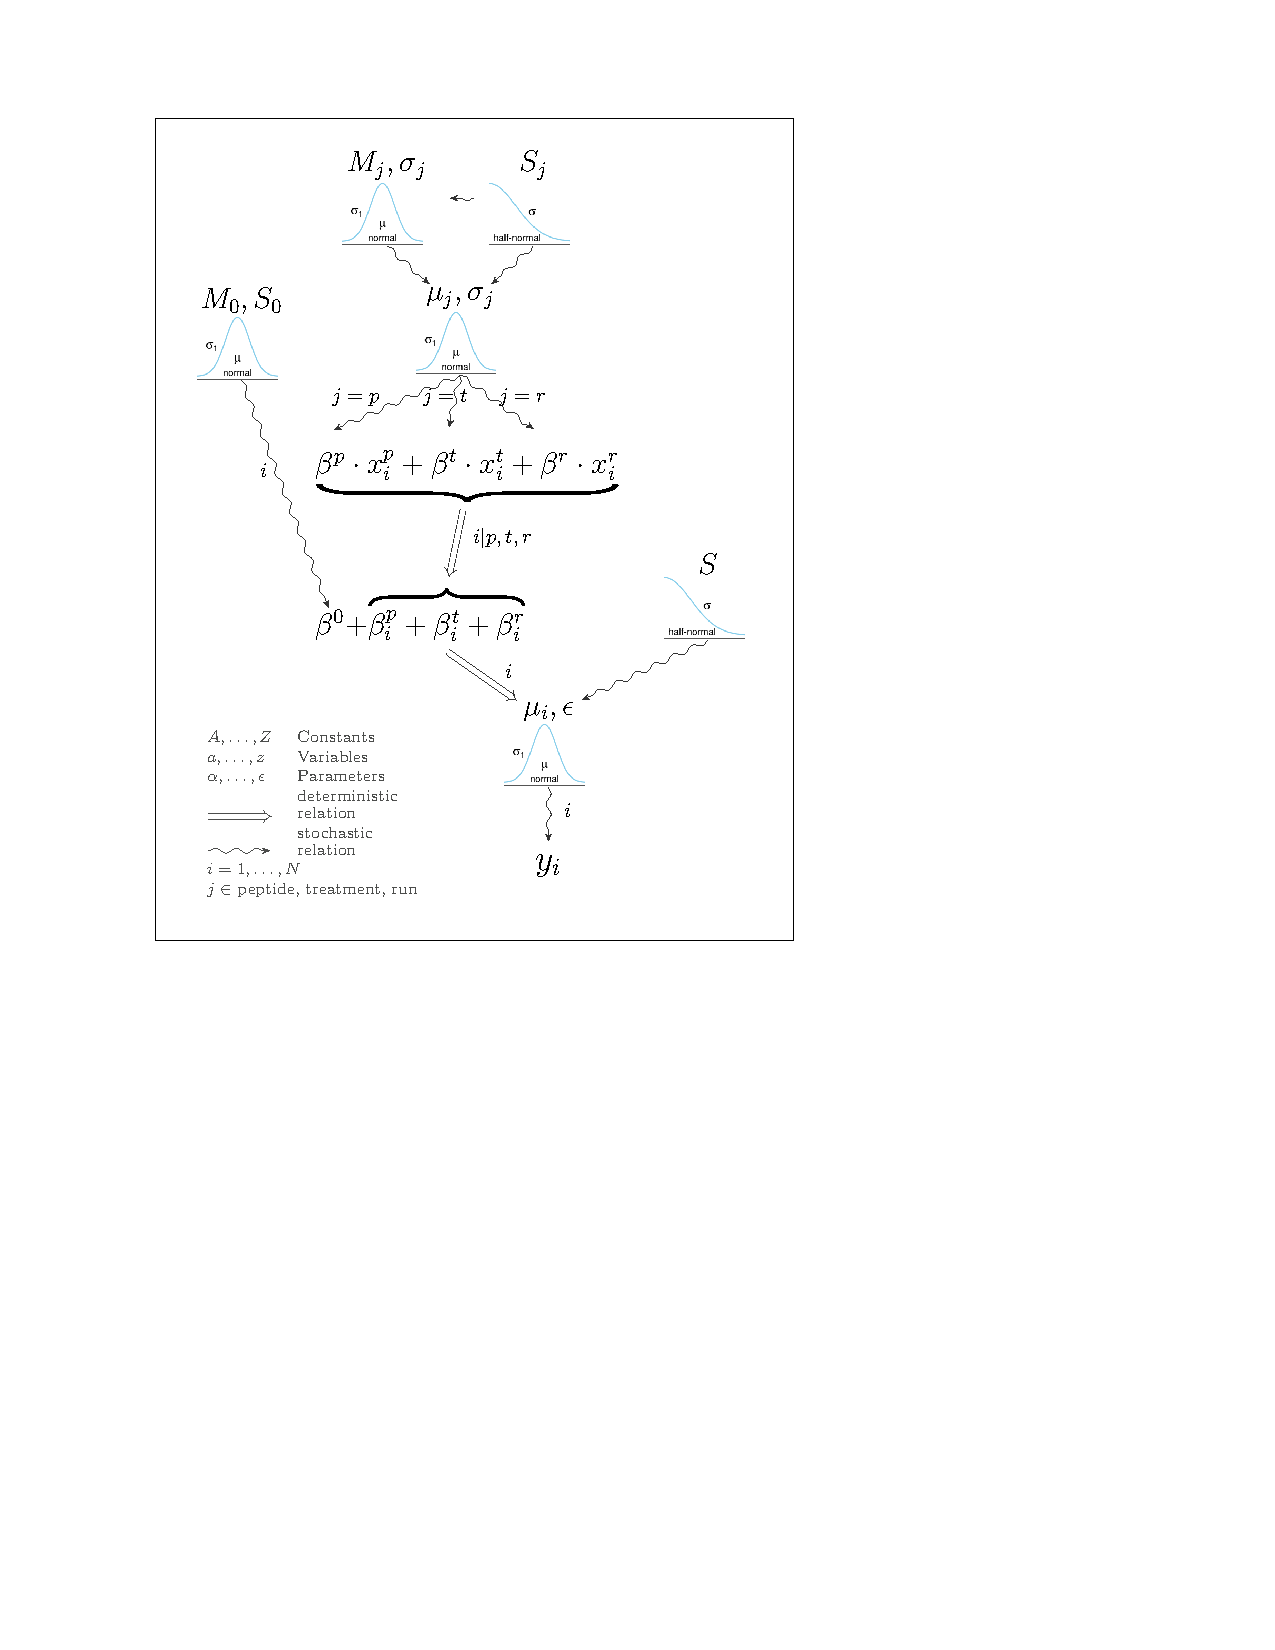
\includepdf[pages=-]{hierarch_diagram.pdf}
\end{figure}


\subsection{Running BayesQuant}

BayesQuant takes a peptide\_summary\_intensity\_moFF\_run.tab (moFF) or a peptides.txt file (MaxQuant) as input, containing a peptide per row. Preprocessing using the MSqRob \texttt{preprocess\_MSnSet()} function, as well as other data munging functions, is required.

%--peptide_file> <--filetype> <--exp_annotation> [--annotation_df] [--organisms] [--protein_file] [--extract_features]

\begin{minted}[mathescape,
               linenos,
               numbersep=5pt,
               obeytabs=true,tabsize=2,
               frame=lines,
               framesep=2mm]{R}

Rscript prepare_BayesQuant.R --pepf peptides.txt \
    --filetype MaxQuant --exp exp_annotation.tsv \
    --output .
\end{minted}

The R script outputs the input file for BayesQuant. Its data is introduced in BayesQuant via the following code:

\begin{minted}[mathescape,
               linenos,
               numbersep=5pt,
               obeytabs=true,tabsize=2,
               frame=lines,
               framesep=2mm]{python}

# Load the module
from BayesQuant import BayesQuant
bayesquant = BayesQuant()
# Read the dataset
bayesquant.read_data(data="ms1_intensities.tsv")
# Compile a model for proteins with 3 peptides
model = bayesquant.compile_model(n_peptides=3)
# Load a specific protein
bayesquant.load_data("A6NDG61")
\end{minted}

The snippet above loads the program, reads in the data, selects the data for a specific protein, and builds a model that matches the number of peptides observed. The posterior distribution can be computed using pure MCMC or VI methods, as stated in section \ref{subsec:posterior_compute}. The VI procedure will now be explained, due to its significantly better performance.

\begin{minted}[mathescape,
               linenos,
               numbersep=5pt,
               obeytabs=true,tabsize=2,
               frame=lines,
               firstnumber=last,
               framesep=2mm]{python}
# VI approximation: much faster and pretty accurate
trace_advi = bayesquant.fit(model_name=p, n_draws=40000)
\end{minted}

The \texttt{bayesquant.fit()} function carries out two tasks:

\begin{itemize}
\item Finds the best mean-field approximation $q(\theta)$ to the true posterior $p(\theta|x)$. This approximate distribution is easier to work with.
\item Sample from the approximate posterior, returning a collection of samples called trace.
\end{itemize}

The values stored in the trace obtained via VI will follow an approximation to the true posterior, and contain the results of the modelling process. Once it is obtained, the inference is complete and model checking ought to be performed to validate the results as explained in section \ref{subsec:model_checking}. It is run with:

\begin{minted}[mathescape,
               linenos,
               numbersep=5pt,
               obeytabs=true,tabsize=2,
               frame=lines,
               firstnumber=last,
               framesep=2mm]{python}
# Run Posterior Predictive Checks
bayesquant.ppc()
\end{minted}

A step by step exposition of the plots and results produced by the program when ran on the proteins  P0A818 (\textit{E. coli}) and A6NDG6 (\textit{Homo sapiens}) will follow.

\subsection{VI optimisation evaluation}


\begin{figure}[H]
%\begin{adjustbox}{varwidth=\textwidth,fbox,center}
\begin{subfigure}{.45\textwidth}
\centering
\caption*{A}
\includegraphics[width=.9\linewidth]{ELBO/P0A8I8}
\end{subfigure}
\begin{subfigure}{.45\textwidth}
\centering
\caption*{B}
\includegraphics[width=.9\linewidth]{ELBO/A6NDG6}
\end{subfigure}
%\end{adjustbox}
\caption[ELBO progression]{Progression of \ac{ELBO} maximisation during the \ac{VI} approximation for proteins P0A818 (\textit{E. coli}, \textbf{A}) and A6NDG6 (\textit{Homo sapiens}, \textbf{B}) over 40k iterations.}
\label{fig:ELBO}
\end{figure}

After the \texttt{.fit()} method is run, a plot of the maximisation of the \ac{ELBO} is produced automatically. Even though the ELBO took extremely low (negative) values at start (see figure \ref{fig:ELBO}), it was maximised fast to values around 0, indicating that the mean-field approximation was acceptably good.


\subsection{Sampling from the approximation to the posterior}
\label{subsec:basic_model}


The 10k traces produced by BayesQuant from the \ac{VI} approximation function exhibited a clear random walk behaviour, which decreases the posibility that the approximation was wrong. Moreover, the  effects caused by the different peptides and runs were estimated and separated from the overall observed noise, allowing for a better estimation of the \ac{log2FC} (see figure \ref{fig:traceplots}).

\begin{figure}[!h]
%\begin{adjustbox}{varwidth=\textwidth,fbox,center}
\begin{subfigure}{\textwidth}
\centering
\caption*{A}
\includegraphics[width=\linewidth]{traceplots/P0A8I8}
\end{subfigure}
\bigskip
\begin{subfigure}{\textwidth}
\centering
\caption*{B}
\includegraphics[width=\linewidth]{traceplots/A6NDG6}
\end{subfigure}
%\end{adjustbox}
\caption[Traceplots for 2 proteins]{Traceplot of the model fit for proteins P0A818 (\textit{E. coli}, \textbf{A}) and A6NDG6 (\textit{Homo sapiens}, \textbf{B}). The left panel shows the frequency density over the parameter space for several model parameters: (I) the \ac{log2FC} estimate (difference of treatment effects), (II) the effects in the three observed peptides, and (III) the effects in the six available runs. The right panel displays the sampled values from the \ac{VI} approximation stored in the trace.}
\label{fig:traceplots}
\end{figure}

This way, a different posterior distribution was computed for the impact of each "peptide" and "run" in all the measurements collected for each protein.


The study of the \ac{log2FC} posterior probability distribution (see figure \ref{fig:posteriors}) shows the most likely parameter values and empowers Bayesian Null Hypothesis Testing. The 95\% High Probability Density Interval (\ac{HPDI}), which is the narrowest interval containing 95\% of the total probability, indicates the most likely true values of the parameter. Presence or absence of overlap between the 95\% \ac{HPDI} and the Region Of Practical Equivalence (\ac{ROPE}) provides a formal way of discarding a point value of the parameter. The \ac{ROPE} is a small interval considered to be essentually the same as the null value \cite{Kruschke}. In this and all future applications in the thesis, the null value is set to 0, and the interval is given a width of 0.4 on each side.

\begin{figure}[!h]
\centering
\begin{subfigure}{0.8\textwidth}
\caption*{A}
\includegraphics[width=\linewidth]{posteriors/P0A8I8}
\end{subfigure}
\bigskip
\begin{subfigure}{0.8\textwidth}
\caption*{B}
\includegraphics[width=\linewidth]{posteriors/A6NDG6}
\end{subfigure}
\caption[Posteriors for 2 proteins]{Annotated posterior probability distribution for the \ac{log2FC} estimate for proteins P0A818 (\textit{E. coli}, \textbf{A}) and A6NDG6 (\textit{Homo sapiens}, \textbf{B}). The bar height is mapped to the probability mass in the corresponding interval. The 95\% \ac{HPDI} is marked with a black line. The \ac{ROPE} defined as a 0.4 window around 0 is shown in red. A green vertical line marks the expected \ac{log2FC} estimate for \textit{E. coli} proteins ($\log_2(3)$).}
\label{fig:posteriors}
\end{figure}

The analysis indicated that P0Q8I8 (\textit{E. coli}) most likely has a \ac{log2FC} between 1.4 and 1.7, and it\textquotesingle significantly different from 0, as no overlap was observed between \ac{HPDI} and \ac{ROPE}. On the other hand, the human protein was found to acquire a \ac{log2FC} most likely between -0.1 and 0.192. This range is fully contained within the \ac{ROPE}, which indicates that the \ac{log2FC} was practically 0 (see figure \ref{fig:posteriors}).


The posterior predictive checks on both proteins pinpoints that the fitted models captured a data generation process approximating what was observed (see figure \ref{fig:ppc}). The three observed peptides were found to be undistinguishable from the 500 simulated ones.

\begin{figure}[!h]
\centering
\begin{subfigure}{0.8\textwidth}
\caption*{A}
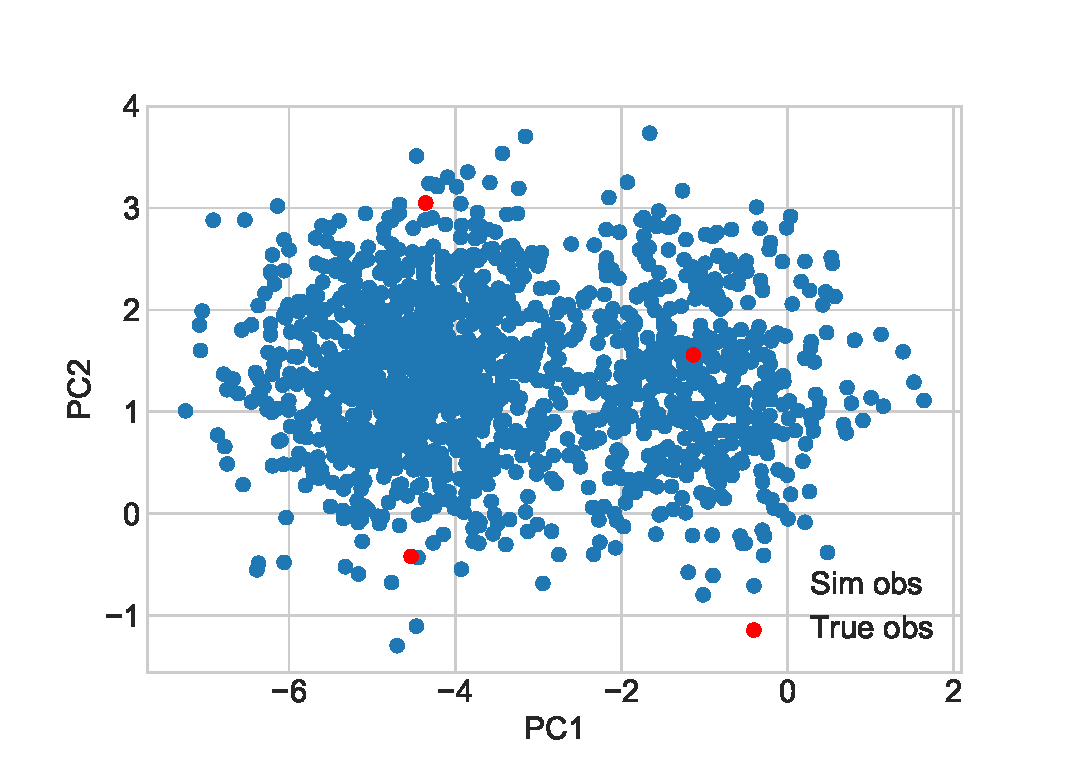
\includegraphics[width=\linewidth]{PPC/eps/PCA_P0A8I8}
\end{subfigure}
\bigskip
\begin{subfigure}{0.8\textwidth}
\caption*{B}
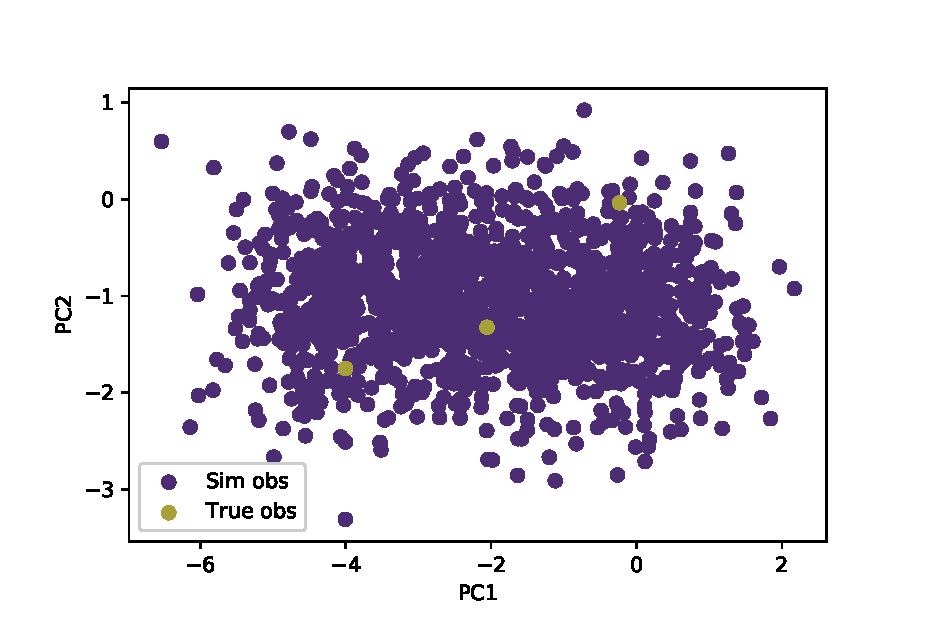
\includegraphics[width=\linewidth]{PPC/eps/PCA_A6NDG6}
\end{subfigure}
\caption[Posterior predictive checks]{Projection of the posterior predictive checks on the 2D plane capturing most variance. Simulated datapoints are shown in blue, whereas actual observations are shown in red.}
\label{fig:ppc}
\end{figure}


In order to further validate BayesQuant\textquotesingle s performance, it was tested on groups of 5 proteins, one group from each proteome. Each pair of groups was made by proteins with a different number of observed peptides (2, 3, 4, 6, 7, 10) (see figure \ref{fig:dumbbell}). The more peptides, the more accurate the estimation will be as more data will be available. Since the \ac{HPDI} reflects the uncertainty, a decrease on its width was expected to be observed (see figure \ref{fig:dumbbell}).

\begin{figure}[!h]
\centering
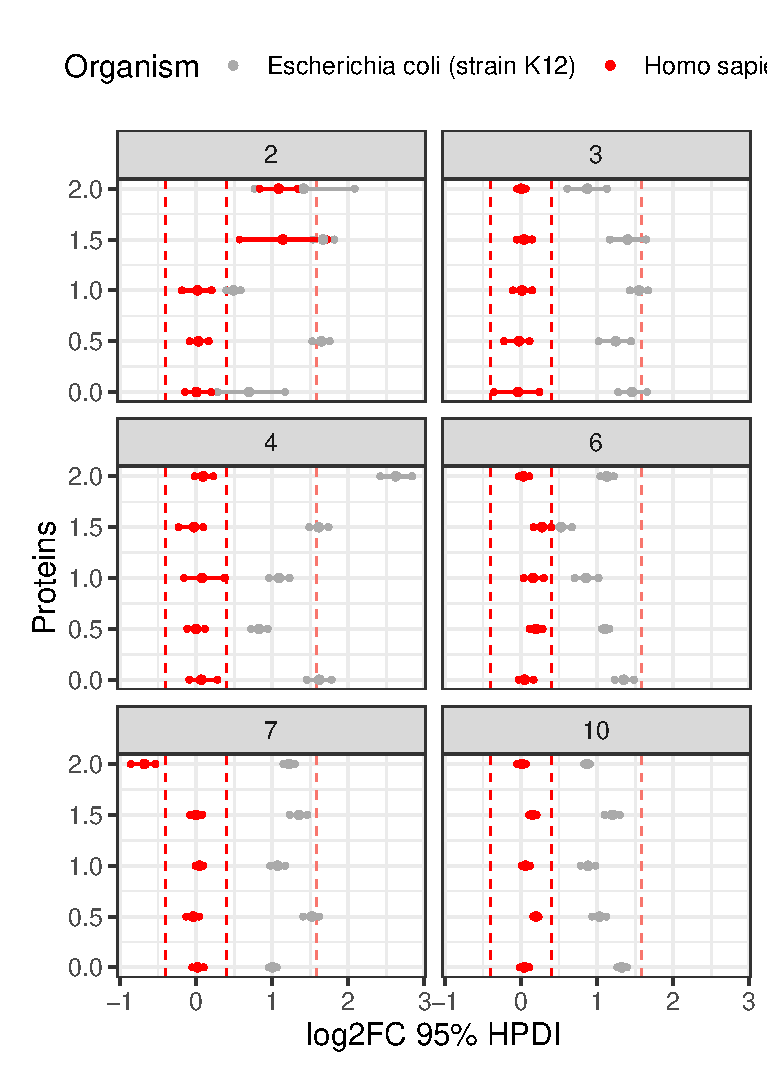
\includegraphics[width=0.9\textwidth]{performance}
\caption[HPDI inferred by BayesQuant]{Visualization of the 95\% \ac{HPDI} inferred from 5 bacterial and 5 human proteins with 2, 3, 4, 6, 7 and 10 peptides. The intervals are represented by horizontal lines. The dot represents the mean of the whole distribution, and it will be centered in the interval if the distribution is symmetrical. Vertical blue lines represent the ROPE defined as in figure \ref{fig:posteriors}, whereas the red line represents the expected estimate for bacterial proteins.}
\label{fig:dumbbell}
\end{figure}


Indeed, a general trend of width reduction was observed with the increased amount of peptides. For example, the widest intervals are observed on proteins with just two peptides available, and the narrowest on proteins with ten. Moreover, the \ac{HPDI} tended to align more strongly around an agreement value as well. 

The consistent observation that \textit{Homo sapiens} proteins got a \ac{log2FC} estimate around 0, and \textit{E. coli} proteins got an estimate which overlapped the predefinned \ac{ROPE} in only three cases (two of which on proteins with two peptides), confirmed the validity of the quantification framework.

\subsection{Extended model: peptide effect with sequence features}
\label{subsec:extended_model}

Given the open-source nature of the program, it is possible to build upon it and extend its functionality. The possibility of making use of the peptide sequences to model the peptide effect using a linear model was considered and put to practice. The code was thus extended with the following snippets of code:

\begin{minted}[mathescape,
               linenos,
               numbersep=5pt,
               obeytabs=true,tabsize=2,
               frame=lines,
               framesep=2mm]{python}

bayesquant.read_data(
    # table with ms1 intensity data
    data_path="data/ms1_intensities.tsv",
    # table with sequence features
    features_path="data/features.tsv")
\end{minted}


\begin{minted}[mathescape,
               linenos,
               numbersep=5pt,
               obeytabs=true,tabsize=2,
               firstnumber=last,
               frame=lines,
               framesep=2mm]{python}

# Specification of priors
sigma_theta = pm.HalfNormal('sigma_theta', sd=1)
theta = pm.Normal('theta', mu=0, sd=sigma_theta, shape = (n_features, 1))
theta_inter = pm.Normal('theta_inter', mu=0, sd=sigma_theta)
mu_pep = pm.Normal("mu_pep",
  mu=theta_inter + pm.math.sum(features.dot(theta)),
  sd=sigma_pep)   
\end{minted}

which means that if the peptide effect is modelled as a function of the sequence, $\mu^p$ is redefined to:

%\begin{align}
%\nonumber \mu^p \sim \mathcal{N}(0, \sigma^p) \, \\
%\end{align}
        
\begin{equation}
\nonumber \sigma^{\theta} \sim \mathcal{HN}(1)
\end{equation}
\begin{equation}
\nonumber \theta_k \sim \mathcal{N}(0, \sigma^{\theta})
\end{equation}
\begin{equation}
\nonumber \mu^p \sim \mathcal{N}(\sum_{k=0}^{k=K}{x_k \theta_k}, \sigma^p)
\end{equation}

where $\theta_k$ is the weight of the $k^{th}$ feature, and $x_k$ is the numerical value of the $k^{th}$ feature. $\sigma^{\theta}$ is the prior for the standard deviation of the Normal all feature weights are sampled from.

The same workflow as in section \ref{subsec:basic_model} was ran with the extended model, and the result is shown in figure \ref{fig:traceplots_seq}. The analysis illustrates the null predictive power of the sequence properties extracted, as all converge extremely strongly to a value of 0. The result is equivalent to not having defined any weights at all, and instead having run the basic model.



\begin{figure}[H]
\begin{subfigure}{\textwidth}
\centering
\caption*{A}
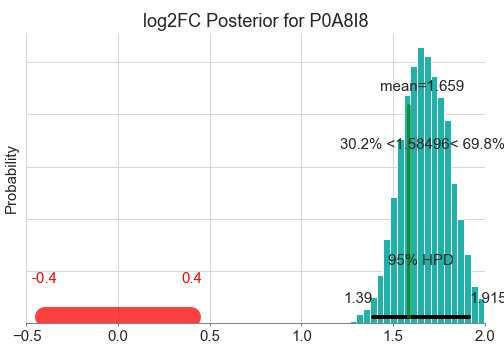
\includegraphics[width=\linewidth]{traceplots/P0A8I8_seq.png}
\end{subfigure}
\bigskip
\begin{subfigure}{\textwidth}
\centering
\caption*{B}
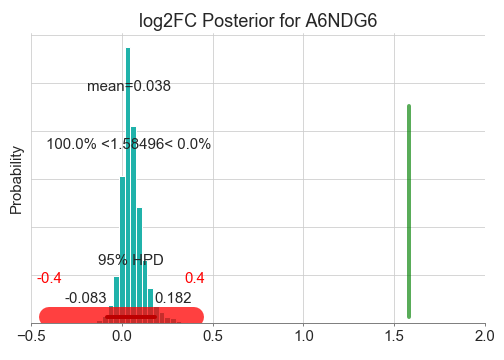
\includegraphics[width=\linewidth]{traceplots/A6NDG6_seq.png}
\end{subfigure}
\caption[Traceplot from sequence modelling of peptide effect]{Traceplot obtained after fitting the extended model on the test proteins mentioned in \ref{subsec:basic_model}. No feature was found to have any predictive power.}
\label{fig:traceplots_seq}
\end{figure}

\section{Discussion}

\subsection{Improving usability: parallelization}

While BayesQuant performed well on the majority of proteins, it took around 30 seconds to approximate each protein\textquotesingle posterior distributions using \ac{VI}, and more than two minutes with \ac{MCMC} methods. This translates to a dataset of 1k proteins taking 500 minutes (>8h) to be processed. However, the average modern computer comes with several processors that could support the parallelization of the program in several threads, decreasing the total computing time.

\subsection{Further robustness and validation checks}

A solid way of checking the results are not flawed is the specification of alternative priors. Unless precise prior knowledge is available, the selection of one prior over another prior to model the beliefs about the system should not have any impact on the results. It is for that reason that models built upon different priors could be run to further validate the program.


\subsection{Advanced model comparison}

Besides the predefinition of a \ac{ROPE} and the check of overlap with the 95 \% \ac{HPDI}, more advanced model comparison methods making use of the Bayes factor are available. The Bayes factor is defined as the ratio of the posterior probability of the models given the data \cite{Kruschke}. It could be used to measure how much more likely a model taking into account a treatment effect is compared to another one where the treatment effect is considered null i.e the \ac{log2FC} is set to 0. The result would provide an alternative criteria for the declaration of a protein being differentially abundant.

\subsection{Sequence-based modelling of the peptide effect}

Unfortunately, during the development of the project, it was acknowledged that the peptide effect is a very difficult phenomenon to capture in a simple Bayesian model as the one presented in this work. This is due to the motley and and multilevel nature of the noise caused by the aminoacidic sequences:

\begin{itemize}

\item The protein neighborhood, which might affect the protease\textquotesingle s efficiency.

\item The competitive ionization problem, introduced in chapter \ref{chap:mass_spec} (\ref{subsec:the_ion_source}) implies that ionization prediction cannot be achieved without models that do not replicate this process mathematically. Thus, the ionization of a peptide ought to be predicted taking into account the peptide mix with which it accessed the ion source as a whole.

%which states that the ionization efficiency of a peptide will not just depend of its sequence, but also of that of its competitors in the ion source. This is due to the ion source providing a limited amount of charges for an excess peptide input. Therefore, a different number of instances of the same peptide acquire charge, depending on how efficient the other peptides simultaneously present are.

\item The mobile proton model \cite{Boyd2010}, which states that the peptide\textquotesingle s fragmentation pattern changes drastically depending on the number of charges and its distribution on the sequence. The charge distribution is hypothesised to be in turn determined by the position of positive residues that can allocate the charges. This phenomenon implies that the \ac{PSM} step is more difficult as a different spectrum is expected for molecules with the same peptide sequence but different charges. The decreased identifications and quality of the peaks makes feature extraction algorithms like the Apex module in moFF would extract worse \ac{MS1} intensities, in turn injecting noise in the quantification data.

\item The characterization of powerful sequence properties that specifically capture the differential ionization efficiency is undone work, as most feature extractors are designed to solve different problems, like protein sructure prediction.

\end{itemize}

Modelling such a complex phenomenon will require accordingly complex predictive architectures and the introduction of proper neural networks, capable of deciphering the intrincate pattern mapping sequence to noise in the spectrometer\textquotesingle s measurements.

\subsection{Posterior assessment of the effects}

The characterization of the uncertainty behind a \ac{log2FC} estimate can be used to better inform downstream analysis programs and eventually help interpret the biological results. For example, a functional analysis program could decide to drop proteins declared differentially abundant if the uncertainty is greater than a threshold. A Gene Set Enrichment Analysis (\ac{GSEA}) could make use of the probabilistic information to refine the results of the enrichment.

Moreover, the estimation of the different run effects could be used to help \ac{MS} technicians assess the presence of batch effects in their experiments, and correct them in future analyses.

\section{Conclusion}

A Bayesian framework for the relative quantification of protein abundance rations (Fold-Change, FC) using \ac{MS1} intensity was presented in this work. Unlike the currently prevailing methods in the field, it provides uncertainty estimates that provide a direct interpretation about the accuracy of the quantification. Moreover, preliminary results on the sequence modelling of the peptide bias revealed that more complex architectures and sequnce features are required to solve this problem. Finally, the method can be used to investigate the presence of batch effects in \ac{MS} experiments for their minimisation in future. While the software can be integrated in any pipeline producing peptide-level data, further testing and improvements are probably required for optimal performance.
